\documentclass[16pt]{article}
\usepackage[russian]{babel}
\usepackage{a4wide}
\usepackage[utf8]{inputenc}
\usepackage{graphicx}
\usepackage{amsmath}
\usepackage{amssymb}
\usepackage{mathrsfs}  
\usepackage{amsthm}
\usepackage{import}
\usepackage{xifthen}
\usepackage{pdfpages}
\usepackage{transparent}
\usepackage{multicol}

\newcommand{\incfig}[2]{%
    \def\svgwidth{#2 mm}
    \import{./figures/}{#1.pdf_tex}
}

\newtheorem{Th}{Теорема}
\newtheorem{Lem}{Лемма}
\newenvironment{Proof}{\par\noindent{\bf Доказательство.}}{\hfill$\scriptstyle\blacksquare$}
\newenvironment{Sol}{\par\noindent{\it Решение:}}


\DeclareMathOperator{\Arccos}{arccos}
\DeclareMathOperator{\Arctg}{arctg}
\DeclareMathOperator{\Cl}{Cl}
\DeclareMathOperator{\Sign}{sgn}
\DeclareMathOperator*{\Argmax}{Argmax}
\DeclareMathOperator*{\Var}{Var}
\DeclareMathOperator*{\Min}{min}


\newcommand\Real{\mathbb{R}} 
\newcommand\A{(\cdot)} 
\newcommand\Sup[2]{\rho( #1 \, | \, #2 )}
\newcommand\Sum[2]{\sum\limits_{#1}^{#2}}
\newcommand\Scal[2]{\langle #1,\, #2 \rangle}
\newcommand\Norm[1]{\left\| #1 \right\|}
\newcommand\Int[2]{\int\limits_{#1}^{#2}}
\newcommand\PS{\mathcal{P}}
\newcommand\X{\mathcal{X}} 
\newcommand\Pict[3]{
\begin{figure}[h!]
    \centering
    \incfig{#1}{#3}
    \caption{#2}
    \label{fig:#1}
\end{figure}
}

\begin{document}

\thispagestyle{empty}

\begin{center}
\ \vspace{-3cm}


\includegraphics[width=0.5\textwidth]{msu.eps}\\
{\scshape Московский государственный университет имени М.~В.~Ломоносова}\\
Факультет вычислительной математики и кибернетики\\
Кафедра системного анализа

\vfill

{\LARGE Отчёт по 3 заданию практикума}

\vspace{1cm}

{\Huge\bfseries <<Достигнуть недостижимого>>}
\end{center}

\vspace{1cm}

\begin{flushright}
  \large
  \textit{Студент 315 группы}\\
  Д.\,М.~Сотников

  \vspace{5mm}

  \textit{Руководитель практикума}\\
  к.ф.-м.н., доцент П.\,А.~Точилин
\end{flushright}

\vfill

\begin{center}
Москва, 2020
\end{center}

\newpage
\section{Постановка задачи}
Для обыкновенного дифференциального уравнения
$$\ddot x + \dot x + 5x^5 + x\sin(x^3) = u, \quad x \in \Real,\ u \in \Real$$
необходимо построить множество достижимости $\X[T] = \X(T, t_0, x(t_0), \dot x(t_0))$ при заданном ограничении
на управление $u \in [-\alpha,\, \alpha]$. Известно, что в начальный момент $t_0 = 0$ состояние
$x(0) = \dot x(0) = 0$. В качестве управлений будем рассматривать измеримые по Лебегу функции $u\A$ такие,
что $|u(t)| \leqslant \alpha$ для почти всех $t$.

Делая замену $x_1 = x, \ x_2 = \dot x$, приводим систему к нормальному виду:
\begin{equation}\label{xsys}
\begin{cases}
\dot x_1 = x_2 \\
\dot x_2 = u - 5x_1^5-x_1\sin(x_1^3)-x_2\\
x_1(0) = x_2(0) = 0
\end{cases}
\end{equation}

\section{Вспомогательные утверждения}
Для решения задачи используется принцип максимума Понтрягина для задачи достижимости, который сформулирован и 
доказан в \cite{LiMarkus} (4.1, теорема 3).

Рассмотрим автономную систему
$$ \dot x(t) = f(x(t), u(t)),$$
дополнительно предполагая, что функции $f, \ \dfrac{\partial f}{\partial x}$ непрерывны, $u\A$ измерима, и 
$u(t) \in \Omega \subset \Real^n$ для почти всех~$t$.

Функция Гамильтона-Понтрягина для $x,\ \psi \in \Real^n$ имеет вид
$$\mathcal{H}(\psi(t), x(t), u(t)) = \Scal{\psi(t)}{f(x(t), u(t))}.$$
\begin{Th}[Принцип максимума Понтрягина]
Пусть $\tilde u\A$ --- допустимое управление, переводящее систему на границу множества достижимости $\X[T]$,
$\tilde x\A$ --- траектория, соответствующая этому управлению, $\tilde x(T) \in \partial \X[T]$. Тогда существует
функция
$\tilde \psi\A  \not\equiv 0$, удовлетворяющая сопряженной системе
$$ \dot \psi = -\dfrac{\partial \mathcal{H}}{\partial x},$$
и выполнено условие максимума
$$\mathcal{H}(\tilde \psi(t), \tilde x(t), \tilde u(t)) \overset{\text{п.в.}}{=} \sup_{v \in \Omega} \mathcal{H}(\tilde \psi(t), \tilde x(t),v).$$
\end{Th}

Из этой теоремы следует, что множество траекторий, удовлетворяющих описанным выше условиям, содержит в себе
все траектории, выводящие систему на границу множества достижимости, поэтому в дальнейшем будут рассматриваться
только траектории и управления, удовлетворяющие принципу максимума.

Вернемся к рассмотрению системы (\ref{xsys}), далее $\psi$ --- сопряженная переменная
из принципа максимума.
Следующая теорема позволяет делать выводы о существовании переключений на некоторых участках траектории.
Она была доказана в \cite{OC}. 

\begin{Th}[о нулях $x_2$ и $\psi_2$]
Пусть $t_1 < t_2$. Тогда, если $x_2(t_1) = x_2(t_2) = 0,$ $x_2$ не обращается в нуль на $(t_1,\,t_2)$, и $\psi_2(t_1) \not= 0$,
то $\psi_2(t_2) \not= 0$, и существует $\tau \in(t_1,\,t_2)$ такая, что $\psi_2(\tau) = 0$.
\end{Th}
Иными словами, между двумя нулямми $x_2$ существует нуль $\psi_2$.
\newpage
\begin{Lem}
В задаче (\ref{xsys}) множество достижимости не убывает в смысле включения, то есть
$$\X(t) \subset \X(t + \Delta t), \quad \forall \Delta t > 0.$$
\end{Lem}
\begin{Proof}
Пусть $a$ --- произвольная точка из $\X(t)$. Покажем, что $a \in \X(t + \Delta t)$.
Так как $a \in \X(t)$, найдется допустимое управление $\overline{u}\A$, определенное на $(0,\, t)$ и
переводящее систему в точку $a$ к моменту
времени $t$. Положим теперь 
$$ u(\tau) = 
\begin{cases}
0, &\tau < \Delta t\\
\overline u(\tau - \Delta t), & \tau \geqslant \Delta t
\end{cases}
$$
Из системы (\ref{xsys}) видно, что система будет оставаться в нуле на отрезке $(0,\, \Delta t)$, затем управление
$\overline u \A$ за время $t$ приведет систему в точку $a$, поскольку система является автономной.
Таким обрзаом $x(t + \Delta t) = a$, а значит, $\ a \in \X(t + \Delta t)$.

\end{Proof}

\section{Применение принципа максимума}
Для данной задачи функционал Гамильтона-Понтрягина имеет вид
$$\mathcal{H} = \psi_1 x_2 + \psi_2(u-5x_1^5-x_1\sin(x_1^3)-x_2),$$
а сопряженная система
\begin{equation}\label{conj}\tag{СС}
\begin{cases}
\dot \psi_1 = \psi_2(25x_1^4 + \sin(x_1^3) + 3x_1^3\cos(x_1^3))\\
\dot \psi_2 = \psi_2 - \psi_1
\end{cases}
\end{equation}

Так как функционал $\mathcal{H}$ линеен по $u$, из условия максимума получаем следующий вид управления:
$$u(t) =
\begin{cases}
\alpha, & \psi_2(t) > 0\\
[-\alpha,\, \alpha], & \psi_2(t) = 0\\
-\alpha, & \psi_2(t) < 0\\
\end{cases}
$$

\begin{Lem}
Особый режим в данной задаче невозможен.
\end{Lem}
\begin{Proof}
Предположим, что $\psi_2(t) = 0$ на некотором отрезке. Тогда на этом же отрезке, в силу постоянства $\psi_2$,
 выполнено $$\dot \psi_2(t) = 0 = \psi_2(t) - \psi_1(t) = -\psi_1(t),$$ а значит, и $\psi_1(t) = 0$ на данном отрезке, 
 что приводит к противоречию с нетривиальностью сопряженной переменной.
\end{Proof}

Итак, управления, приводящие на границу множества, почти всюду принимают максимальные по модулю значения
и имеют вид
$$u(t) = \alpha \Sign( \psi_2(t))$$

Система при этом движется в двух режимах, соответствующих $u = \alpha$ и $u = -\alpha$:

\begin{equation}\label{xsys-}\tag{---}
\begin{cases}
\dot x_1 = x_2 \\
\dot x_2 = -\alpha - 5x_1^5-x_1\sin(x_1^3)-x_2
\end{cases}
\end{equation}


\begin{equation}\label{xsys+}\tag{+}
\begin{cases}
\dot x_1 = x_2 \\
\dot x_2 = \alpha - 5x_1^5-x_1\sin(x_1^3)-x_2
\end{cases}
\end{equation}

\newpage
\section{Алгоритм решения}
Выпустим из начального положения две траектории по системам (\ref{xsys+}) и (\ref{xsys-}).
Заметим, что при $u = \alpha$ переменная $x_2$ сначала возрастает, также возрастает и $x_1$, затем, когда
они достигают некоторого значения, производная $\dot x_2$ становится отрицательной, и в некоторый момент
$x_2$ обращается в нуль. Те же рассуждения приводят к тому, что при $u = -\alpha$ переменная $x_2$
сначала убывает, затем возрастает и обращается в нуль. 

Таким образом при любом значении параметра $\alpha$ данные траектории имеют примерно такой вид:

\begin{figure}[h]\label{pict}
\center
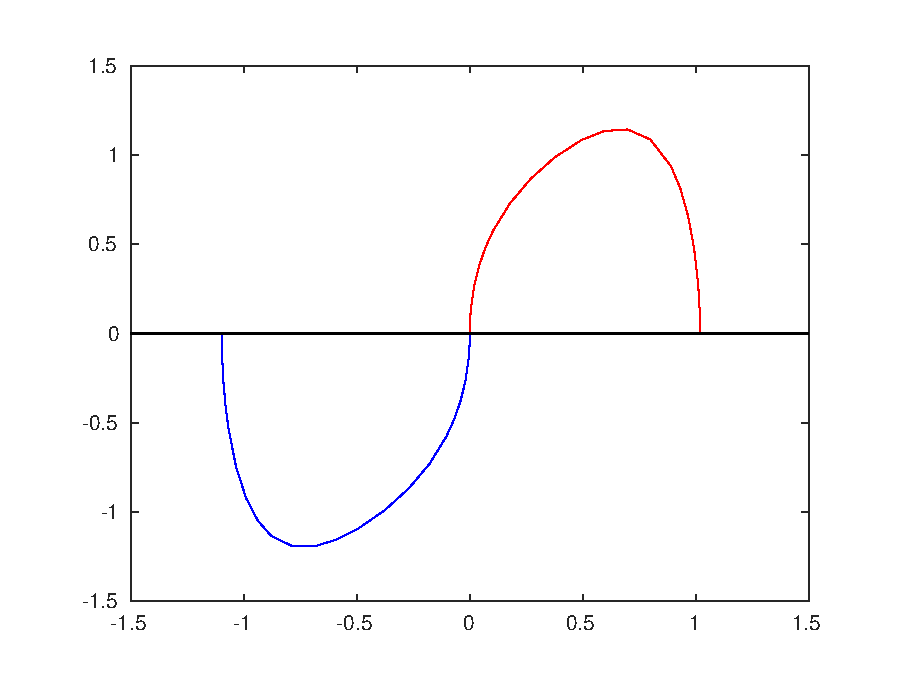
\includegraphics[width=110mm]{start.eps}
\caption{Траектории систем (\ref{xsys+}) и (\ref{xsys-})}
\end{figure}


Значения $\tau_-,\ \tau_+$, при которых $x_2$ обращается в нуль, находятся численно с помощью функции ode45. 

Рассмотрим теперь ветвь $u = \alpha$. По теореме о нулях найдется $\tau_s~\in~(0,\, \tau_+)$~---~нуль функции $\psi_2$, то есть момент переключения. При этом, в силу положительной однородности сопряженной 
переменной в принципе максимума, можно считать, что $|\psi_1(\tau_s)|~=~1$. Так как на $[0,\,\tau_s]$ управление
было положительно, функция $\psi_2$ была так же положительна, и потому прошла через нуль убывая, то есть
$$\dot \psi_2(\tau_s) =-\psi_1(\tau_s) < 0.$$
Отсюда $\psi_1(\tau_s) = 1$. 

В момент $\tau_s$ известны значения всех параметров, поэтому, интегрируя (\ref{xsys-}) и (\ref{conj})
и переключаясь между системами при обращении $\psi_2$ в нуль,
найдем конец траектории $x(T)$.

При численном решении параметр $\tau_s$ перебирается по интервалу $(0,\,\min(T, \tau_+))$.

Абсолютно аналогично рассматривается отрицательная ветвь с единственным отличием: в момент переключения
$\psi_1(\tau_s) = -1$.

Упорядочивая полученное множество конечных точек получим границу множества достижимости. Основной проблемой 
здесь является возниконовение <<острых углов>> на границе при самопересечениях построенной кривой.

Для удаления частей кривой, находящихся внутри множества достижимости, используется следующий алгоритм:
\begin{itemize}
\item Находится точка, лежащая на границе множества достижимости, она становится начальной точкой массива.
Такой точка является, например, точка с наибольшим значением $x_1$.
\item Находятся точки, подозрительные на пересечение (близкие по расстоянию и сильно различающиеся по индексам).
\item Для подозрительных точек $x_i, x_j$ проверяется, пересекаются ли отрезки $[x_{i-1},\,x_{i+1}]$ и
 $[x_{i-1},\,x_{i+1}]$. Если отрезки пересекаются, то участок кривой между подозрительными точками удаляется.
\end{itemize}

Также в программе фиксируются моменты переключений перебираемых траекторий.

\section{Положения равновесия}
Необходимо также проверить возможность прохождения траектории близко к неподвижной точки соответствующей 
системы. Из уравнения $f(x) = 0$ получим уравнение неподвижной точки для системы (\ref{xsys+})
$$
\begin{cases}
x_2 = 0\\
5x_1^5+x_1\sin(x_1^3) = \alpha
\end{cases}
$$
и для системы (\ref{xsys-})
$$
\begin{cases}
x_2 = 0\\
5x_1^5+x_1\sin(x_1^3) = -\alpha
\end{cases}
$$

\begin{figure}[h]
\begin{multicols}{2}
	\hfill
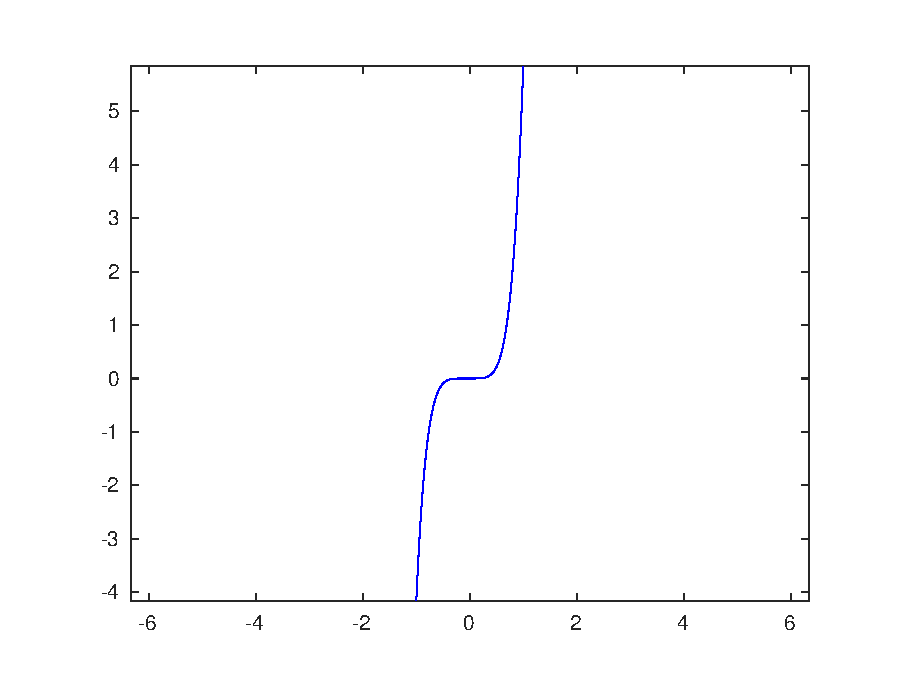
\includegraphics[width=80mm]{eq.eps}
	\hfill
\caption{График $5x^5 + x\sin(x^3)$}
	\hfill
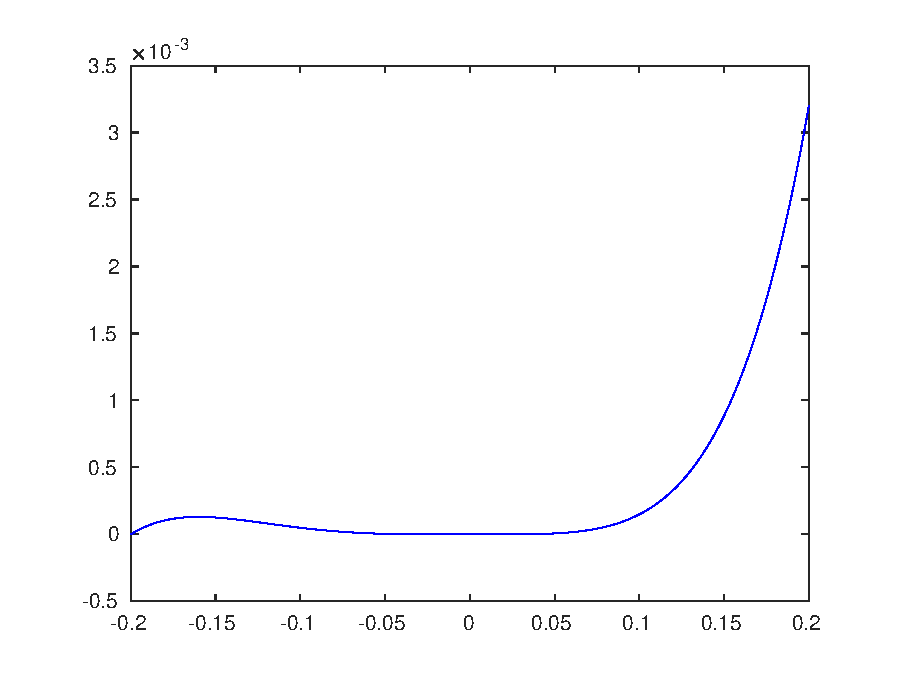
\includegraphics[width=80mm]{eq2.eps}
	\hfill
\caption{График $5x^5 + x\sin(x^3)$}
    \hfill
\end{multicols}
\end{figure}
Из графика видно, что при значениях $\alpha > 0.0002$ система (\ref{xsys+}) имеет положение равновесия с $x_1^* > 0$,
а система (\ref{xsys-}) имеет равновесие с $x_1^* < 0$. Обозначим $f(x) = 5x^5 + x\sin(x^3)$. Заметим, что в системе
(\ref{xsys+}) на красной траектории на рис.1
$$\dot x_2 = \alpha - f(x_1^*) - x_2 = -x_2 < 0$$
Это означает, что вектор $f(x_1^*, x_2)$ сонаправлен с вектором $[1,\, -1]^T$, что возможно только
на участке $t \in (0,\, \tau_+)$, поскольку далее $\dot x_1 < 0$. Но точка на $(0,\, \tau_+)\times \{0\}$
будет лежать в зоне, где после переключения система будет двигаться в режиме (\ref{xsys-}), а значит, при
вычислении её можно не учитывать. Второе положение равновесия обрабатывается аналогично.

При малых $\alpha \leqslant 0.0002$ у положительной системы будет существовать положение равновесия с $x_1^* < 0$,
однако этот корень на несколько порядков больше $\alpha$, и потому множество достижимости, которое будет
равномерно ограничено по времени (числом порядка $\sqrt{\alpha}$), не достигнет данной точки.

\section{Примеры работы}
Рассмотрим эволюцию множества достижимости при $\alpha = 1$. Здесь и далее красным и синим отмечены кривые
первых трех переключений.


\begin{figure}[h]
\begin{multicols}{2}
	\hfill
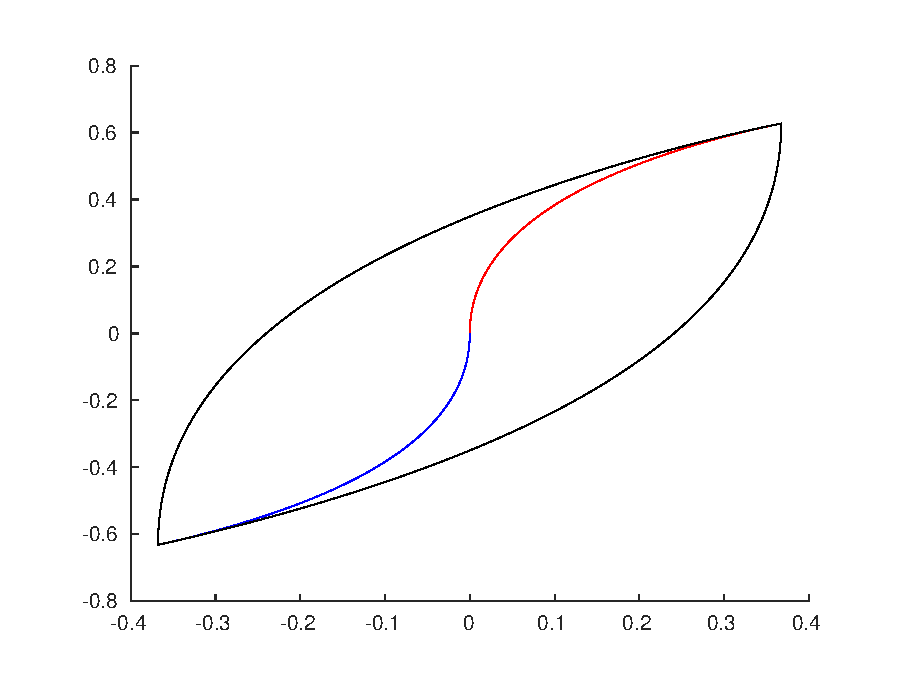
\includegraphics[width=80mm]{1_1.eps}
	\hfill
\caption{$T = 1$}
	\hfill
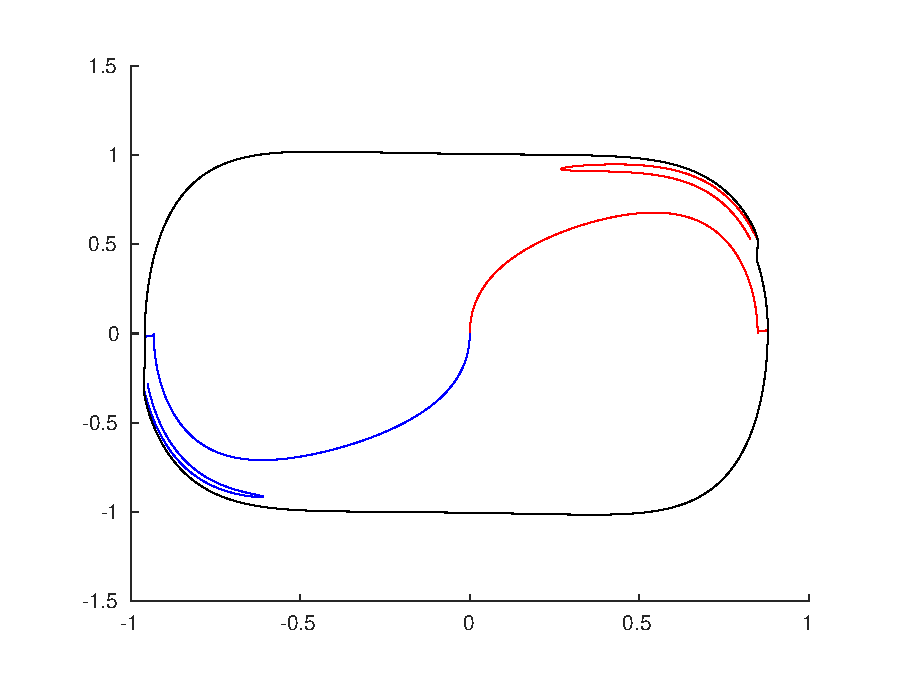
\includegraphics[width=80mm]{4_1.eps}
	\hfill
\caption{$T = 4$}
    \hfill
\end{multicols}
\end{figure}



\begin{figure}[h]
\center
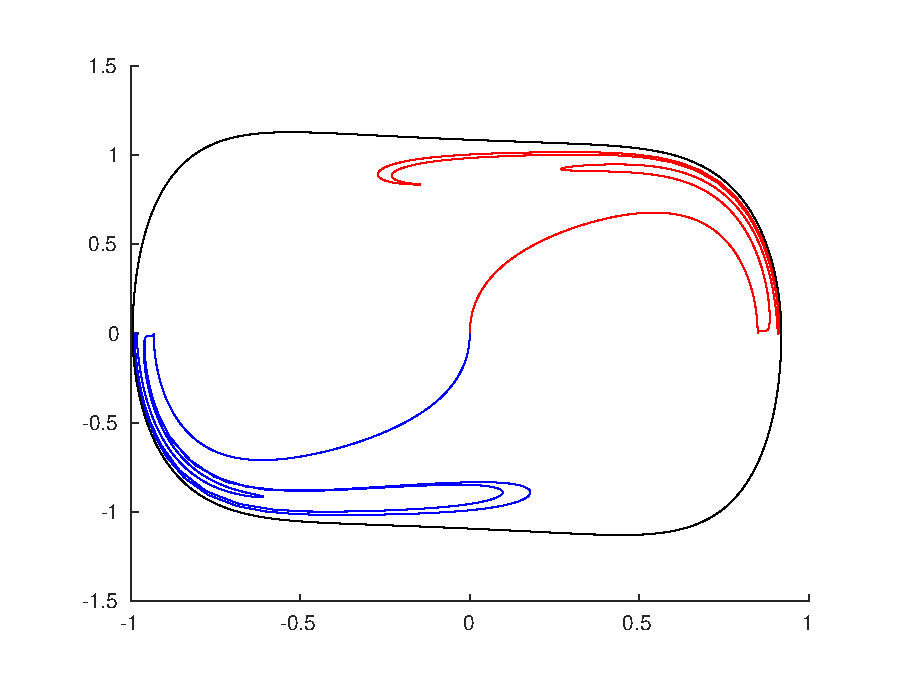
\includegraphics[width=80mm]{10_1.eps}
\caption{$T = 10$}
\end{figure}
\newpage

Видно, что множество достижимости растет, стремясь к некоторому ограниченному предельному множеству.

Еще несколько примеров при других значениях параметров:


\begin{figure}[h]
\begin{multicols}{2}
	\hfill
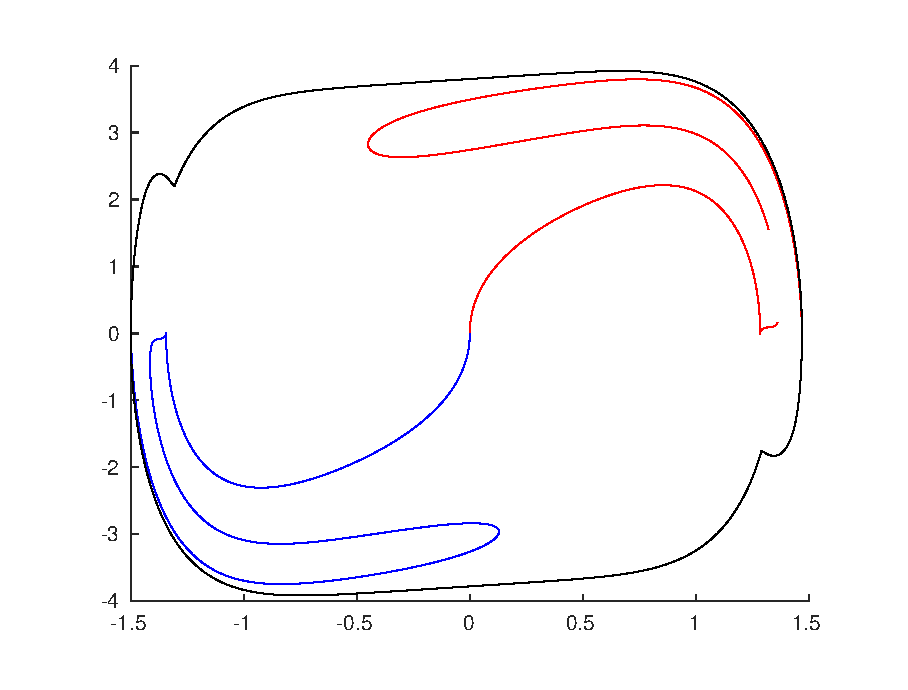
\includegraphics[width=80mm]{19_5.eps}
	\hfill
\caption{$T = 1.9,\ \alpha = 5$}
	\hfill
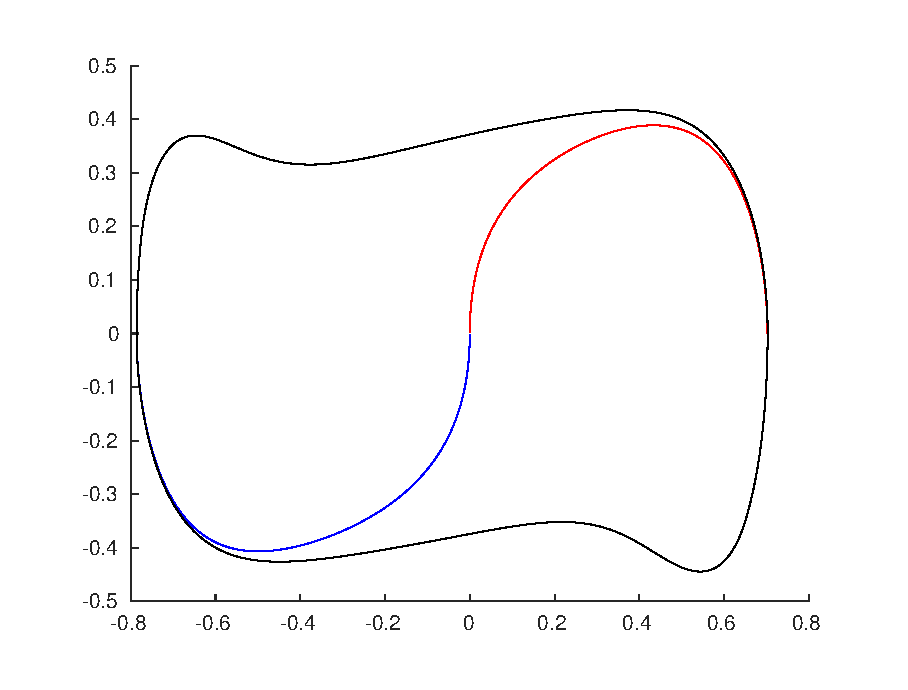
\includegraphics[width=80mm]{3_05.eps}
	\hfill
\caption{$T = 3,\ \alpha = 0.5$}
    \hfill
\end{multicols}
\end{figure}

\newpage
\begin{thebibliography}{0}
\bibitem{OC}
	Комаров~Ю.А. Лекции по оптимальному управлению. ВМК МГУ, 2020. 
\bibitem{LiMarkus}
	Ли~Э.Б., Маркус Л. Основы теории оптимального управления. --- М.: Наука, 1972.
\end{thebibliography}


\end{document}
